\subsection{THE LARGEST NILPOTENCY IDEAL OF A REPRESENTATION}

Lemma 2. Let \(\mathfrak{g}\) be a Lie algebra, \(\mathfrak{a}\) an ideal of \(\mathfrak{g}\) and \(\mathbf{M}\) a simple \(\mathfrak{g}\) -module. If, for all \(x \in \mathfrak{a}\) , \(x_{\mathbf{M}}\) is nilpotent, then \(x_{\mathbf{M}} = 0\) for all \(x \in \mathfrak{a}\) .

Let \(\mathbf{N}\) be the subspace of \(\mathbf{M}\) consisting of the \(m \in \mathbf{M}\) such that \(x_{\mathbf{M}}.m = 0\) for all \(x \in \mathfrak{a}\) . By Theorem 1, \(\mathrm{N} \neq \{0\}\) . On the other hand, for all \(y \in \mathfrak{g}\) , \(\mathbf{N}\) is stable under \(y_{\mathbf{M}}\) (§ 3, no. 5, Proposition 5). Hence \(\mathbf{N} = \mathbf{M}\) , which proves the lemma.

Lemma 3. Let \(\mathfrak{g}\) be a Lie algebra, a an ideal of \(\mathfrak{g}\) , M a \(\mathfrak{g}\) -module of finite dimension over

K and \((\mathbf{M}_{i})_{0\leqslant i\leqslant n}\) a Jordan-Hölder series of the g-module M. The following conditions are equivalent:

\begin{enumerate}
\def\labelenumi{(\alph{enumi})}
\item
  for all \(x \in a\) , \(x_{M}\) is nilpotent;
\item
  for all \(x \in \mathfrak{a}\) , \(x_{\mathbf{M}}\) is in the Jacobson radical of the associative algebra \(\mathbf{A}\) generated by 1 and the \(y_{\mathbf{M}}\) where \(y \in \mathfrak{g}\) ;
\item
  for all \(x \in a\) ,
\end{enumerate}

\[
x _ {\mathrm{M}} \left(\mathrm{M} _ {0}\right) \subset \mathrm{M} _ {1}, x _ {\mathrm{M}} \left(\mathrm{M} _ {1}\right) \subset \mathrm{M} _ {2}, \dots , x _ {\mathrm{M}} \left(\mathrm{M} _ {n - 1}\right) \subset \mathrm{M} _ {n}.
\]

If these conditions are fulfilled, a is orthogonal to g with respect to the bilinear form associated with the g-module M.

\begin{enumerate}
\def\labelenumi{(\alph{enumi})}
\setcounter{enumi}{1}
\item
  \(\Rightarrow\) (a): as A is finite-dimensional over K, the Jacobson radical of A is a nilpotent ideal (Algebra, Chapter VIII, § 6, no. 4, Theorem 3) and hence every element of this radical is nilpotent.
\item
  \(\Rightarrow\) (c): each \(Q_{i} = M_{i}/M_{i+1}\) ( \(0 \leqslant i < n\) ) is a simple g-module. For all \(x \in \mathfrak{a}\) , the endomorphism \(x_{Q_{i}}\) (which is derived from \(x_{M}\) by restricting to \(M_{i}\) and passing to the quotient) is nilpotent if condition (a) holds and hence zero by Lemma 2; in other words, \(x_{M}(M_{i}) \subset M_{i+1}\) .
\item
  \(\Rightarrow\) (b): suppose condition (c) holds; let \(x\in\mathfrak{a}\) and \(z\in\mathrm{A}\) . Then \(z(\mathrm{M}_{i})\subset\mathrm{M}_{i}\) ( \(0\leqslant i<n\) ) and hence \((zx_{\mathrm{M}})^{n}(\mathrm{M})=\{0\}\) ; thus \(\mathrm{Ax}_{\mathrm{M}}\) is a left nilideal of A and hence is contained in the Jacobson radical of A (Algebra, Chapter VIII, § 6, no. 3, Corollary 3 to Theorem 1).
\end{enumerate}

Finally, suppose conditions (a), (b) and (c) hold. Let \(x \in \mathfrak{a}\) and \(y \in \mathfrak{g}\) . We have just seen that \(y_{\mathbb{M}}x_{\mathbb{M}}\) is nilpotent and hence \(\operatorname{Tr}(y_{\mathbb{M}}x_{\mathbb{M}}) = 0\) , which proves the last assertion of the lemma.

PROPOSITION 4. Let \(\mathfrak{g}\) be a Lie algebra, M a \(\mathfrak{g}\) -module of finite dimension over K and A the associative algebra generated by 1 and the set of \(x_{\mathbf{M}}\) ( \(x \in \mathfrak{g}\) ).

\begin{enumerate}
\def\labelenumi{(\alph{enumi})}
\item
  The ideals \(\mathfrak{a}\) of \(\mathfrak{g}\) such that \(x_{\mathbf{M}}\) is nilpotent for all \(x \in \mathfrak{a}\) are all contained in one of them, \(\mathfrak{n}\) .
\item
  The ideal n is the set of \(x \in g\) such that \(x_{M}\) belongs to the Jacobson radical of A.
\item
  Let \((\mathrm{M}_{i})_{0\leqslant i\leqslant n}\) be a Jordan-Hölder series of the g-module M; then n is also the set of \(x \in g\) such that \((x)_{\mathrm{M}_{i}/\mathrm{M}_{i+1}} = 0\) for all i.
\item
  n is orthogonal to g with respect to the bilinear form associated with ρ.
\end{enumerate}

The set of \(x \in \mathfrak{g}\) such that \(x_{\mathbf{M}}\) belongs to the Jacobson radical of \(\mathbf{A}\) is obviously an ideal of \(\mathfrak{g}\) . The proposition then follows immediately from Lemma 3.

DEFINITION 2. The ideal n of Proposition 4 is called the largest nilpotency ideal for the g-module M or the largest nilpotency ideal of the corresponding representation.

\pandocbounded{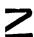
\includegraphics[keepaspectratio]{images/part001_a9d92cc3.jpg}}

Clearly n contains the kernel of this representation. It equals it when M is semi-simple (Proposition 4 (c)), but not in general. It should be noted that an element x of g such that \(x_{M}\) is nilpotent does not necessarily belong to n.

We also note that a particular case of Lemma 3 immediately gives the following result:

PROPOSITION 5. Let \(\mathbf{V}\) be a vector space of finite dimension \(n\) over \(\mathbf{K}\) and \(g\) a Lie subalgebra of \(\mathfrak{gl}(\mathbf{V})\) whose elements are nilpotent endomorphisms of \(\mathbf{V}\) . Then there exists a decreasing sequence of vector subspaces \(\mathrm{V}_0, \mathrm{V}_1, \ldots, \mathrm{V}_n\) of \(\mathbf{V}\) , of dimensions \(n, n - 1, \ldots, 0\) , such that \(x(\mathrm{V}_i) \subset \mathrm{V}_{i+1}\) for all \(x \in g\) and \(i = 0, 1, \ldots, n - 1\) .

